\section{Fællesoffentlig referencearkitektur for deling af data og
dokumenter}\label{fuxe6llesoffentlig-referencearkitektur-for-deling-af-data-og-dokumenter}

\emph{Versionsoversigt:}

\emph{Version 0.1, september 2017. Arbejdsdokument, der bygger oven på
en tidligere udarbejdet Synopsis for Referencearkitektur for deling af
data og dokumenter (august 2017). Benyttet i workshop med
arkitektarbejdsgruppen under SDA.}

\emph{Version 0.2, primo oktober 2017. Arbejdsdokument benyttet i
forbindelse med anden workshop med arkitektarbejdsgruppen under SDA.}

\emph{Version 0.3, medio oktober 2017. Opdateret med input fra Workshop
2. Udgør Delleverance 2 ift. projektet Referencearkitektur for deling af
data og dokumenter.}

\section{Resume}\label{resume}

Hverdagen er digital, og data om borgere, virksomheder, myndigheder,
ejendomme, steder, køretøjer o.m.m. vedligeholdes i en lang række
områder af den offentlige administration. Der ligger et stort potentiale
i at gøre sådanne data tilgængelige for genbrug, så de kan skabe værdi i
andre sammenhænge end formålet med det oprindelige register. Dette kan
danne fundament for langt bedre understøttelse af tværgående, offentlige
services, og åbner tillige for anvendelse af data i nye og innovative
sammenhænge.

Men deling af data kan være teknisk kompliceret og i mange tilfælde
omkostningstungt, bl.a. drevet af krav til sikkerhed og dermed bevarelse
af borgeres og virksomheders tillid til datadeling i det offentlige
Danmark. Derfor er potentialet i deling og genbrug af data i høj grad
forblevet uindfriet.

Denne referencearkitekturs formål er at hjælpe med at indfri dette
potentiale. Dette gøres ved at introducere en fælles beskrivelse af de
begreber og sammenhænge, der er væsentlige for at forstå og arbejde med
design og implementering af løsninger, der involverer deling af data og
dokumenter. Dette sker både på det strategiske plan, hvor vision, mål og
arkitektoniske principper fastlægges; på det forretningsmæssige plan,
hvor de typiske brugsscenarier beskrives; og på det tekniske plan, hvor
en række implementeringsmønstre angiver, hvordan man i og mellem
applikationer kan dele og forsende data.

Referencearkitekturen er udarbejdet under den fællesoffentlige
digitaliseringsstrategi 2016-2020 og er som sådan relevant for alle
offentlige myndigheder og deres leverandører samt for virksomheder, der
ønsker at gøre brug af offentlige data.

\section{Introduktion}\label{introduktion}

\subsection{Formål og målgruppe}\label{formuxe5l-og-muxe5lgruppe}

Referencearkitekturen for deling af data og dokumenter understøtter
design, udvikling og anvendelse af offentlige it-systemer, der

\begin{itemize}
\tightlist
\item
  (gen)anvender oplysninger i form af data og dokumenter til
  sagsbehandling eller selvbetjening
\item
  sender eller modtager meddelelser fra andre it-systemer
\end{itemize}

Dokumentet er primært målrettet it-arkitekter tilknyttet offentlige
digitaliseringsprojekter, herunder enterprise-arkitekter,
forretningsarkitekter og løsningsarkitekter, der har til opgave at
kravspecificere og designe løsninger.

De første dele af dokumentet (Strategisk og Forretningsmæssig
arkitektur) henvender sig endvidere til projektledere og
beslutningstagere, herunder forretningsansvarlige,
digitaliseringschefer, it-chefer, afdelings- og kontorchefer og andre
med rollen som systemejer.

Dokumentet i sin helhed er også relevant for leverandører at orientere
sig i.

\subsection{Scope}\label{scope}

Referencearkitekturen beskriver anvendelse af og udvikling af
it-systemer, der reguleres af blandt andet:

\begin{description}
\tightlist
\item[EU databeskyttelse]
\emph{lov} som beskriver pligter og rettigheder ved behandling af
persondata
\item[EU eIDAS]
\emph{lov} som definerer registrede tillidstjenester
\item[Persondatalov]
\emph{lov} som beskriver pligter og rettigheder ved behandling af
persondata
\item[Lov om Digital Post]
\emph{lov} der gør det obligatorisk for virksomheder og borgere at
modtage digitale meddelelser fra offentlige afsendere.
\end{description}

Referencearkitekturen skrives på baggrund af den fællesoffentlige
digitaliseringsstrategi 2020 under initiativ 8.1 med tilslutning fra FM,
UFM, EVM, SIM, JM, EFKM, MBUL, SÆM, SKM, MFVM, BM, KL og Danske
Regioner. Heri beskrives referencearkitekturen således:

\begin{quote}
For at operationalisere, hvilke krav hvidbogen konkret stiller til
initiativer og systemer udarbejdes en referencearkitektur for deling af
data og dokumenter, der blandt andet beskriver fælles behovsmønstre og
mønstre for teknisk understøttelse, herunder de forskelige roller, der
skal afklares i initiativerne. Referencearkitekturen udpeger også
eventuelle områder for eksisterende og nye fælles standarder og
infrastruktur, som skal lette initiativernes implementering.
Referencearkitekturen bliver således en generel ramme og støtte for alle
initiativernes egen specifikke arkitektur.
\end{quote}

Uden for scope af denne referencearkitektur er:

\begin{itemize}
\tightlist
\item
  registrering og intern anvendelse af data hos registerejer
\item
  åbne data, der ikke kræver adgangskontrol (se issue \#9)
\item
  streaming (se issue \#2)
\end{itemize}

\subsection{Centrale begreber}\label{centrale-begreber}

I det efterfølgende vil begrebet data blive brugt til at betegne både
oplysninger på dokumentform og oplysninger der optræder i registre. Vi
anvender begrebet datasamling både om et register og et repository med
dokumenter.

\begin{figure}
\centering
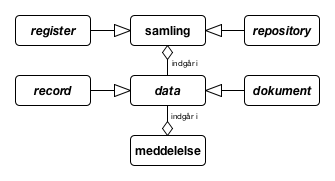
\includegraphics{figures/abstraktion.png}
\caption{Anvendelse af begrebet data og relaterede begreber i denne
referencearkitektur}
\end{figure}

Vi vil endvidere lave en skelnen mellem:

\begin{itemize}
\tightlist
\item
  Anvendelse af udstillede data - typisk via API i
  system-til-system-integrationer
\item
  Forsendelse af meddelelser indeholdende data (herunder dokumenter) -
  typisk brugt ved beskeder til borgere/virksomheder, der skal have
  retsvirkning, men også et klassisk mønster brugt i
  system-til-system-integrationer.
\end{itemize}

Den fundamentale forskel på disse to scenarier er, om det er afsenderen
eller modtageren af data, der kender formålet med interaktionen. Ved
udstilling af data er dataafsenderen som udgangspunkt ikke bekendt med
datamodtagerens formål (men er naturligvis forpligtet til at håndhæve
relevant hjemmel). Ved forsendelse af meddelelser er det dataafsenderen,
der i en given kontekst afsender en meddelelse med et givent formål -
typisk som led i en proces.

\subsection{Anvendelse}\label{anvendelse}

Referencearkitekturen skal:

\begin{itemize}
\tightlist
\item
  danne et fælles sprog til at formulere en fælles handlingsplan
\item
  bruges som reference ved løsningsbeskrivelser
\end{itemize}

\subsection{Tilblivelse og governance}\label{tilblivelse-og-governance}

Første udgave er skrevet hos Kontor for Data og Arkitektur af Mads
Hjorth, Digitaliseringsstyrelsen og Anders Fausbøll, Omnium Improvement.

Endelig godkendelse forventes hos Styregruppe for Data og Arkitektur
under Digitaliseringsstrategien 18. december 2017.

\subsection{Metoderamme}\label{metoderamme}

Referencearkitekturen er udarbejdet inden for rammerne af
Fællesoffentlig Digital Arkitektur og følger så vidt muligt den fælles
skabelon for referencearkitekturer som udarbejdet i DIGST/KDA.
Metoderammen bygger blandt andet på erfaringer fra OIO
referencearkitektur, og indarbejder også elementer fra EIRA, TOGAF,
ArchiMate m.m.

I dokumentets tekst er særlige elementer angivet i \emph{kursiv} (fx
\emph{lov}, \emph{mål}, \emph{rolle} m.m.). Dette markerer, at de hører
til Archimate-begrebsapparatet. Andre elementer er angivet med særlig
\texttt{markering}. Her er der tale om referencer til begreber/elementer
fra figurer. Det bemærkes, at prefixet `data-' kan være udeladt på
begreber/elementer i tekst og figurer fx af formatterings- eller
læsbarhedshensyn uden, at der ligger en indholdsmæssig skelnen bag (fx
\texttt{dataanvendelse}/\texttt{anvendelse},
\texttt{datasamling}/\texttt{samling} o.a.)

I figurer markerer: - \emph{Kursiv}: At et element eller en relation
ikke er nærmere defineret i denne rammearkitektur (fx \emph{dokument}) -
Blå tekst: At et element eller en relation ejes og defineres i denne
rammearkitektur (fx \texttt{anvendelse})

\subsection{Relation til andre
referencearkitekturer}\label{relation-til-andre-referencearkitekturer}

Denne referencearkitektur gør brug af:

\begin{itemize}
\tightlist
\item
  Fællesoffentlig referencearkitektur for brugerstyring
\end{itemize}

Den skal kunne anvendes af:

\begin{itemize}
\tightlist
\item
  Fællesoffentlig referencearkitektur for selvbetjening
\item
  Fællesoffentlig referencearkitektur for overblik over egne sager og
  ydelser
\end{itemize}

\ldots{} og skal anvendes i kontekst sammen med:

\begin{itemize}
\tightlist
\item
  Deling af dokumenter på sundhedsområdet
\item
  Sag- og dokument på det kommunale område
\item
  Indberetning til registre på sundhedsområdet (under udarbejdelse pr.
  oktober 2017)
\end{itemize}

\section{Strategisk arkitektur}\label{strategisk-arkitektur}

Udarbejdelsen af referencearkitekturen tager udgangspunkt i en række
identificerede forretningsmæssige og teknologiske trends og tendenser.

\subsection{Forretningsmæssige
tendenser}\label{forretningsmuxe6ssige-tendenser}

\begin{itemize}
\tightlist
\item
  Nationalt ønske om at undgå knopskudte løsninger
\item
  Data har øget værdi for organisationer
\item
  Øget bevågenhed omkring beskyttelse af privatliv
\item
  Øget opmærksomhed om håndtering af personlige oplysninger
\item
  Mængden af oplysninger der håndteres stiger
\item
  Grænseoverskridende services
\end{itemize}

\subsection{Teknologiske tendenser}\label{teknologiske-tendenser}

\begin{itemize}
\tightlist
\item
  øget central standardisering af begreber, datamodeller og grænseflader
\item
  Flere og mere forskelligartede enheder forbundet til netværket
\item
  Øgede forventninger til brugervenlighed af offentlige digitale
  services
\item
  Mængden af tilgængelige oplysninger vokser
\item
  Arkitekturvision for anvendelse og udstilling
\item
  Integrated Service Delivery
\item
  ''Interoperability/Samarbejdende infrastrukturer / Økosystem af fælles
  løsninger?''
\item
  ''Valgfrihed for anvender mellem flere tekniske udbydere af samme
  oplysninger''
\end{itemize}

\subsection{Strategiske
målsætninger}\label{strategiske-muxe5lsuxe6tninger}

De overordnede målsætninger for denne referencearkitektur kobler alle
til visionen om det datadrevne samfund, hvor data ses som et råstof for
samfundsudviklingen.

Målsætningerne inkluderer:

\begin{description}
\tightlist
\item[Interoperabilitet]
\emph{mål} om sammenhængende services\ldots{} integrated service
delivery
\item[Once-only]
\emph{mål} om at borger og virksomhed kun skal afgive den samme
information til det offentlige en gang\ldots{} (men give lov til
genbrug?)
\item[Transparens]
\emph{mål} om at borgere og virksomheder skal kunne se, hvilke data der
findes om dem, og hvor disse data anvendes
\item[Genbrug]
\emph{mål} om genbrug af it med henblik på lavere omkostninger
\end{description}

\subsection{Vision}\label{vision}

Visionen i denne referencearkitektur er at stræbe efter en situation,
hvor:

\begin{quote}
\emph{Data er en fælles, værdifuld og velbeskyttet ressource, som skal
være nemme at dele og bruge, men svære at misbruge}
\end{quote}

\begin{quote}
\emph{Borgere og virksomheder har overblik over deres data og i hvilke
sammenhænge, de anvendes}
\end{quote}

\subsection{Værdiskabelse}\label{vuxe6rdiskabelse}

Værdien ved at følge denne referencearkitektur er, at den giver:

\begin{itemize}
\tightlist
\item
  Mindre besvær for borger og virksomheder ved brug af digitale services
\item
  Simplere arbejdsgange og mere potentiale for automatisering hos
  organisationer (myndigheder/virksomheder)
\item
  Understøttelse af værdiskabende innovation (ved at gøre data til et
  `råstof' for vækst/skabelse af konkurrencefordele)
\item
  Understøttelse af transparens og dermed bevarelse af tillid til
  registre
\item
  Effektiv systemudvikling (begrænser udfaldsrum, opsamler best
  practice)
\end{itemize}

\subsection{Strategiske principper}\label{strategiske-principper}

Forretningsmæssige, Informationsmæssige, Applikationsmæssige og Tekniske
principper bag referencearkitekturen:

\begin{itemize}
\tightlist
\item
  F1: Byrden i datadeling skal afløftes fra dataejer, hvis den begrænser
  genbrug
\item
  F2: Autoritative registre med henvisninger til andre registre
\item
  F3: Ansvar for begrænsning af adgang ligger hos registerejer
\item
  F4: Data beskrives, fordeles, forbedres og beskyttes i fællesskab
\item
  F5: Beskrivelse af, adgang til og brug af data sker under klar
  governance og håndhæves ud fra tydelig hjemmel
\item
  I1: Fælles referenceinformationsmodel
\item
  I2: Dokument-princip (attester mv.)?
\item
  A1: Onlineopslag i sagsbehandling og selvbetjening
\item
  A2: Log adgang
\item
  A3: Adgang til og fra internationale registre sker gennem national
  gateway
\item
  T1: Central fuldmagts-/rettighedsstyring
\item
  T2: Multi-flavour-api
\item
  T3: Fælles metoder for datadeling understøtter sammenstilling af data
  og tværgående brug blandt myndigheder og virksomheder
\end{itemize}

\section{Forretningsmæssig
arkitektur}\label{forretningsmuxe6ssig-arkitektur}

\subsection{Aktører}\label{aktuxf8rer}

De væsentligste aktører, der er i spil omkring deling af data og
dokumenter, er:

\begin{itemize}
\tightlist
\item
  Offentlige myndigheder, herunder virksomheder, der handler på vegne af
  offentlige myndigheder
\item
  Borgere
\item
  Virksomheder
\end{itemize}

\subsection{Forretningstjenester og
funktioner}\label{forretningstjenester-og-funktioner}

Forretningsmæssigt set finder referencearkitekturen anvendelse i
løsningen af alle offentlige opgaver. Specifikt kan nævnes nedenstående
sæt af generiske procesmønstre:

\begin{itemize}
\tightlist
\item
  Myndigheders sagsbehandling (fra Referencearkitektur for Sag og
  dokument)
\item
  Selvbetjening, vendt mod borgere og virksomheder (fra
  Referencearkitektur for Selvbetjening)
\item
  Indsigt i oplysninger og deres anvendelse (fra Referencearkitektur for
  Overblik over sag og ydelser)
\item
  Sende meddelelse (inkl. brug af tilmeldingslister og påmindelser)
\item
  Modtage meddelelse
\item
  Tag et dokument med til en anden service provider, der ikke har adgang
  til registre - herunder beskrive, hvordan dokumenter valideres.
\item
  Tværgående analyse, tilsyn og kontrol
\end{itemize}

Referencearkitekturen kredser om fire centrale, delte \emph{use cases},
hvor aktører arbejder sammen i forskellige roller.

\begin{figure}
\centering
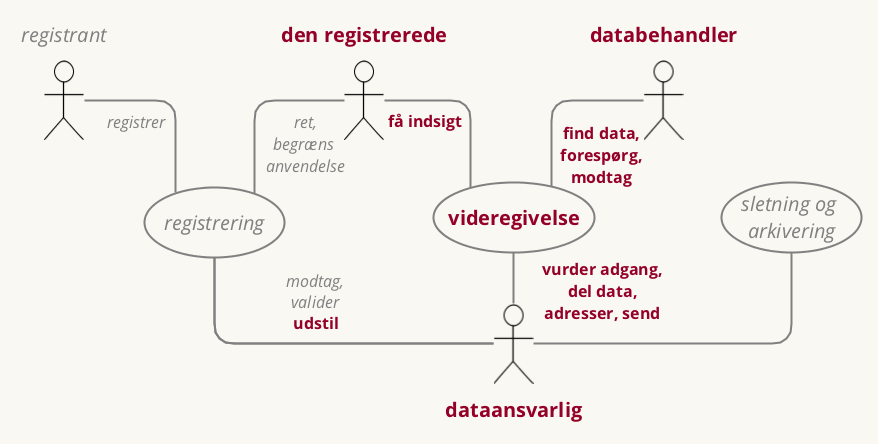
\includegraphics{figures/forretningsroller.png}
\caption{Tværgående use cases og funktioner hos de enkelte roller}
\end{figure}

De fire use cases er:

\begin{description}
\tightlist
\item[Registrering]
\emph{collaboration} hvor oplysninger bringes på digital form
\item[Indsigt i anvendelse]
\emph{collaboration} hvor en borger får indsigt i anvendelse af
personlige data
\item[Anvendelse (af udstillede data, herunder dokumenter)]
\emph{collaboration} hvor oplysninger anvendes i en opgave
\item[Registreret forsendelse]
\emph{collaboration} hvor meddelelser sendes uafviseligt
\end{description}

\subsection{Forretningsroller}\label{forretningsroller}

I ovenstående use cases indgår disse forretningsroller:

\begin{description}
\tightlist
\item[Registrant]
\emph{rolle} som bringer oplysninger på digital form, registrer
\item[``Den registrerede'']
\emph{rolle} den person (datasubjekt), som oplysningerne vedrører
\item[Anvender]
\emph{rolle} der anvender data/oplysninger fra et register
\item[Dataansvarlig]
\emph{rolle} som ejer registreringer/data og har ansvar for at udarbejde
adgangspolitik
\item[Afsender]
\emph{rolle} som genererer og afsender meddelelser til en specifik
modtager
\item[Modtager]
\emph{rolle} som modtager en meddelelse fra en specifik afsender
\end{description}

\subsection{Tværgående processer}\label{tvuxe6rguxe5ende-processer}

\begin{figure}
\centering
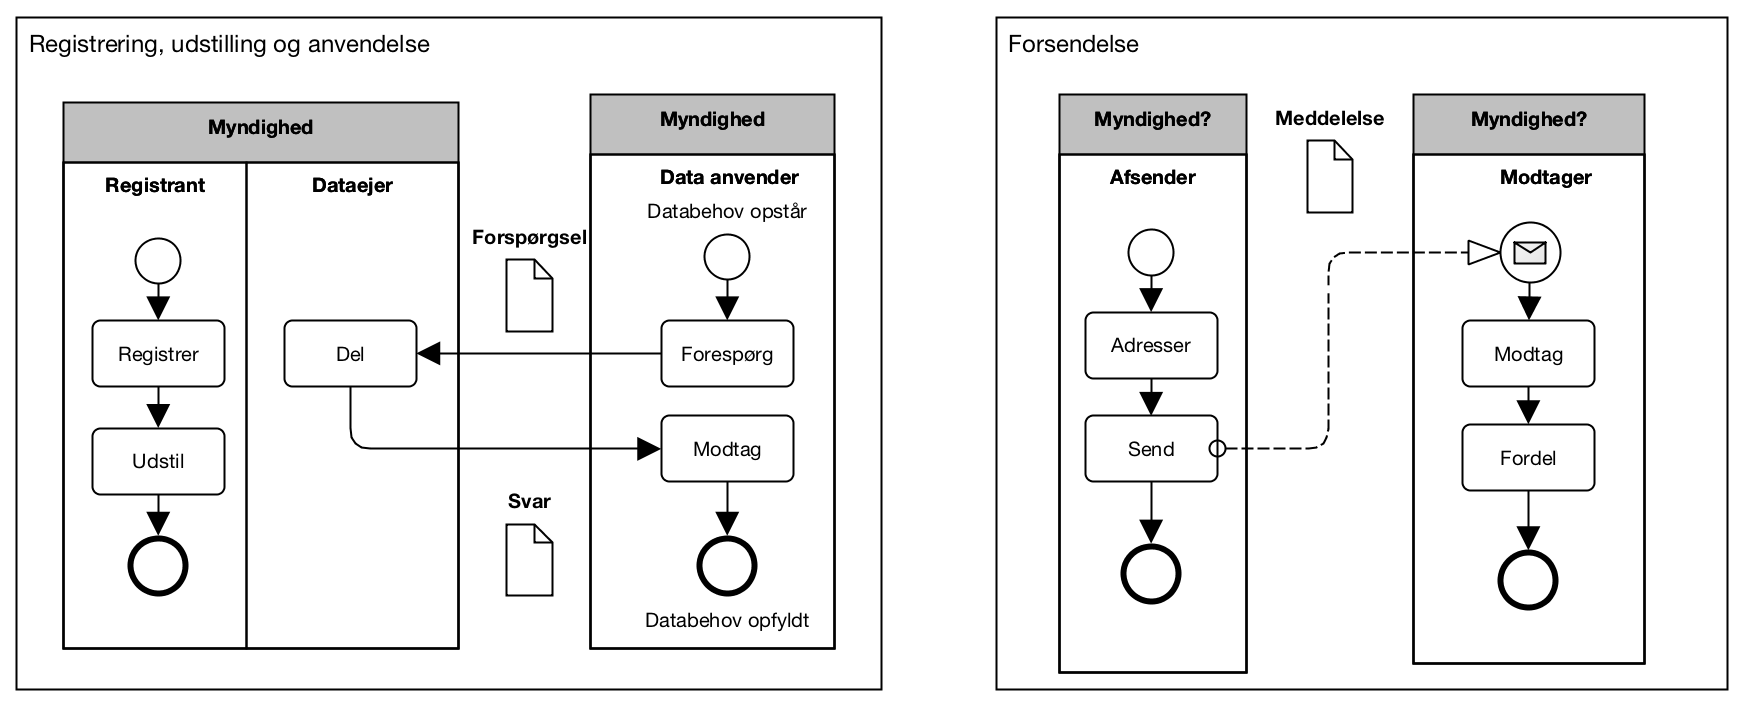
\includegraphics{figures/patterns.png}
\caption{Overblik over centrale processer og deres aktiviteter fordelt
på roller}
\end{figure}

Figuren ovenfor beskriver de væsentligste trin i de overordnede
procesflow for de fire delte use cases. I denne sammenhæng skal følgende
fremhæves:

\begin{description}
\tightlist
\item[Registrering]
\emph{proces} En \texttt{registrant} initierer processen ved at
registrere ny data hos den \texttt{dataansvarlige} (der er ansvarlig for
sikring af hjemmel og håndhævelse af adgangspolitik ifm.
registreringen). Når data er korrekt registreret, skal det markeres som
klar til at blive udstillet. Her kan der være forskel på, om data gøres
tilgængeligt øjeblikkeligt eller først på et senere tidspunkt (fx ved
registrering af fremtidigt skift af adresse) - begge muligheder kan være
relevante, afhængig af \texttt{dataanvenders} behov.
\item[Indsigt i anvendelse]
\emph{proces} \emph{- beskrivelse TBU}
\item[Anvendelse af udstillede data]
\emph{proces} Denne proces initieres hos \texttt{dataanvender} - typisk
en myndighed, men kan også være en virksomhed - ud fra en startsituation
defineret ved, at man har erkendt et behov for data.
\texttt{Dataanvender} sender en forespørgsel på data, der beskriver
dels, hvilke data, der ønskes, og dels med hvilken hjemmel.
\texttt{Dataansvarlig} håndhæver på denne baggrund adgangskontrol, inden
data deles og sendes i et svar til \texttt{dataanvender}.
Slutsituationen bliver, at \texttt{dataanvenders} databehov er opfyldt.
\texttt{Dataansvarlig} er ikke nødvendigvis klar over, hvilket databehov
forespørgslen har tjent til at tilfredsstille - så længe, adgangen er
legitim og foretaget på baggrund af gyldig hjemmel, kender
\texttt{dataansvarlig} ikke nødvendigvis formålet med
\texttt{dataanvenders} brug af data i den konkrete forespørgsel.
\item[Registreret forsendelse]
\emph{proces} Til forskel fra Anvendelse af udstillede data starter
denne proces hos \texttt{afsenderen} (der tillige kan være
\texttt{dataansvarlig}). \texttt{Afsender} har udvalgt og pakketeret
data i en meddelelse (evt. helt eller delvist i form af et dokument),
adresserer meddelelsen (fx ved brug af et kontaktregister) og sender den
herefter til \texttt{modtager}. \texttt{Modtager} kan være alle typer af
aktører; for myndigheder og virksomheder bemærkes, at det i forbindelse
med modtagelsen kan være relevant at fordele/route meddelelsen internt
ud fra dens adresseringsoplysninger. I sammenligning med Anvendelse af
udstillede data er det nu \texttt{afsender}, der som den part, der deler
data, `ejer' den fulde forretningskontekst - hvor den
\texttt{dataansvarlige} ovenfor ikke var bekendt med formålet med at
dele data.
\end{description}

\subsection{Forretningsobjekter}\label{forretningsobjekter}

Nedenfor fremgår en initiel oversigt over en række forretningsobjekter,
der er væsentlige for referencearkitekturen.

\emph{Regibemærkning for version 0.3: Det videre arbejde skal klarlægge,
hvilke elementer der skal indgå i listen, samt hvordan de defineres.
Modelleringsniveauet skal endvidere lægges fast (begrebsmodellering
og/eller logiske kernemodeller?) Kommentarer og midlertidige
bemærkninger indgår i listen, markeret med kantede parenteser.}

\begin{figure}
\centering
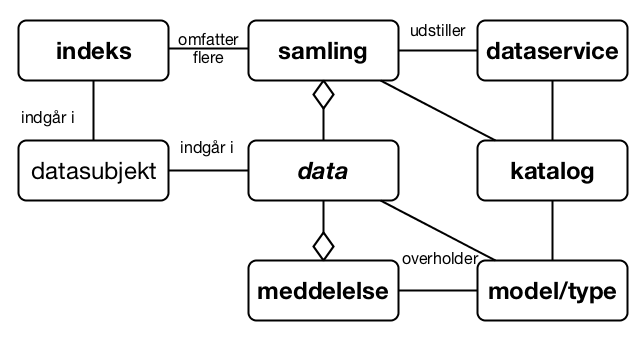
\includegraphics{figures/objekter.png}
\caption{Oversigt over de centrale forretningsobjekter og deres
relationer}
\end{figure}

\begin{description}
\tightlist
\item[data]
\emph{objekt} (Abstrakt. Bruges om både register-record og dokument)
\item[samling]
\emph{objekt} {[}Datasætmodel har ikke definition\ldots{}{]} ISO9115: en
identificerbar samling af oplysninger (samlebetegnelse for PSI, GPDR, )
\item[meddelelse]
\emph{objekt} {[}NgDP{]} registreret forsendelse
\item[datasubjekt]
\emph{objekt} {[}Grunddata, fx person. GPDR: den registrede{]}
\item[model/type]
\emph{objekt} {[}Jf. modelregler fra FDA{]}
\item[katalog]
\emph{objekt} {[}jf hvidbog{]} både data, service\ldots{} til design
\item[dataservice]
\emph{objekt} webservice med adgang til datasamling
\end{description}

og andre mulige

\begin{description}
\tightlist
\item[registeroplysning]
\emph{objekt} en record
\item[dokument]
\emph{objekt} {[}Dokumentmodel fra OIO{]}
\item[påmindelse]
\emph{objekt} {[}Næste generation Digital Post{]}
\item[registreringshændelse]
\emph{objekt}
\item[forretningshændelse]
\emph{objekt}
\item[klassifikation]
\emph{objekt}
\end{description}

\section{Teknisk arkitektur}\label{teknisk-arkitektur}

Dette afsnit beskriver roller og implementeringsmønstre, der er
relevante, når forretningsfunktionerne beskrevet ovenfor skal
understøttes/realiseres af applikationer. Endvidere udpeges områder, der
er kandidat til standardisering og/eller profilering i forbindelse med
referencearkitekturen.

\subsection{Applikationsroller}\label{applikationsroller}

De nødvendige og understøttende applikationsroller og deres indbyrdes
relationer er vist i figuren nedenfor. Nødvendige roller udbyder det
minimale sæt af services, der er i spil i en datadelingsarkitektur.
Undersøttende roller udbyder services, der i mange situationer vil være
fordelagtige at implementere for at øge tilgængelighed, performance,
brugervenlighed m.m. i en given datadelingsløsning.

\begin{figure}
\centering
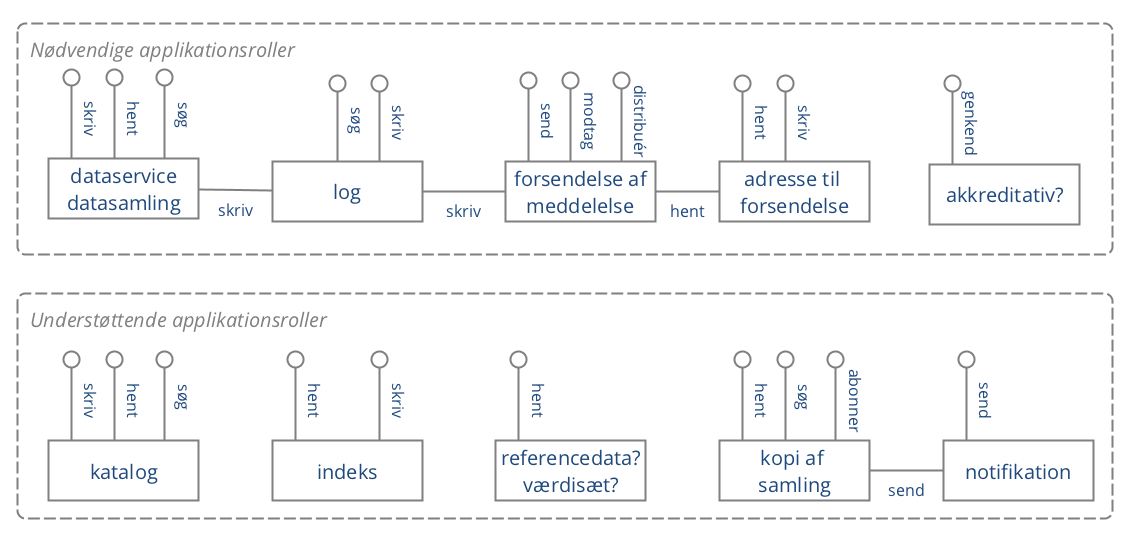
\includegraphics{figures/applikationsroller.png}
\caption{Oversigt over nødvendige og understøttende applikationsroller}
\end{figure}

\begin{description}
\tightlist
\item[Datasamling (dataservice?)]
\emph{applikationsrolle} som har til ansvar at opbevare en
\texttt{datasamling}, udstille denne og begrænse adgangen til den om
nødvendigt
\end{description}

Når datasamlingen udgøres af dokumenter kaldes den nogle gange et
repository, ellers kaldes den også et register. Data kan skrives og
fremsøges igen ved opslag. \texttt{Samlinger} kan have temporale og
bitemporale egenskaber. Dette handler blandt andet om at holde styr på
datas gyldighedsperiode og registreringstidspunkt for fx at kunne
understøtte dobbelt historik (overblik både over, hvad der var korrekt
på en given dato, og hvad registeret på et givent tidspunkt troede var
korrekt på samme tidspunkt).

(Record Management og Data Publication i EIRA)

\begin{description}
\tightlist
\item[Log (adgangslog? anvendelseslog?)]
\emph{applikationsrolle} en slags datasamling, der indeholder
oplysninger om videregivelse af data fra datasamlinger
\end{description}

Der findes også andre typer af logs, fx skrive-log og validerings-log. I
denne sammenhæng er fokus på logning af de data, som en registreret har
ret til at få oplyst.

(Logging, EIRA)

\begin{description}
\tightlist
\item[Forsendelse]
\emph{applikationsrolle} der kan modtage og distribuere meddelelser
\end{description}

(Messaging og Registered Electronic Delivery, EIRA)

\begin{description}
\tightlist
\item[Adresse]
\emph{applikationsrolle} en slags datasamling (fx et kontaktregister),
der indeholder oplysninger til brug ved adressering af meddelelser
\end{description}

(Capability Lookup og Service Discovery, EIRA)

\begin{description}
\tightlist
\item[Id/Rettighed (Brugerstyring?)]
\emph{applikationsrolle} der anvendes til identifikation af brugere og
tildeling af rettigheder (?)
\end{description}

(Identity Management og Access Management, EIRA)

\begin{description}
\tightlist
\item[Katalog]
\emph{applikationsrolle} en slags datasamling, der beskriver en given
\texttt{datasamling}. Anvendes typisk på design-tidspunktet.
\end{description}

Der findes kataloger over mange ting: services, datasæt, systemer,
datamodeller, dokumenttyper\ldots{}

\begin{description}
\tightlist
\item[Indeks]
\emph{applikationsrolle} en slags datasamling, der indeholder
oplysninger om, hvilke datasamlinger der indeholder oplysninger om
personer, virksomheder og andre forvaltningsobjekter. Et Indeks har
typisk til formål at effektivise søgning og fremfinding
\item[Kopi]
\emph{applikationsrolle} en datasamling, som er en direkte kopi af den
\texttt{dataansvarliges} autoritære datasamling
\end{description}

Den kan have en abonnementsservice, så \texttt{anvender} kan abonnere på
ændringer i datasamlinger.

(Data Publication Service i EIRA)

\begin{description}
\tightlist
\item[Notifikation]
\emph{applikationsrolle} der udsender notifikationer/påmindelser.
\end{description}

(Messaging, EIRA)

\begin{description}
\tightlist
\item[Portal]
\emph{applikationsrolle} der udstiller digital selvbetjening rettet mod
en særlig målgruppe, fx borgere eller virksomheder
\end{description}

\subsection{Tekniske Implementeringer}\label{tekniske-implementeringer}

Her grupperes de enkelte forretningsroller og applikationsroller i
forskellige implementeringsmønstre.

\subsubsection{Anvendelse af udstillede
data}\label{anvendelse-af-udstillede-data}

Når en \texttt{dataanvender} (virksomhed eller myndighed) vil have
adgang til data hos en dataansvarlig myndighed, kan det ske via ét af
nedenstående tre mønstre:

\paragraph{Direkte adgang}\label{direkte-adgang}

\begin{figure}
\centering
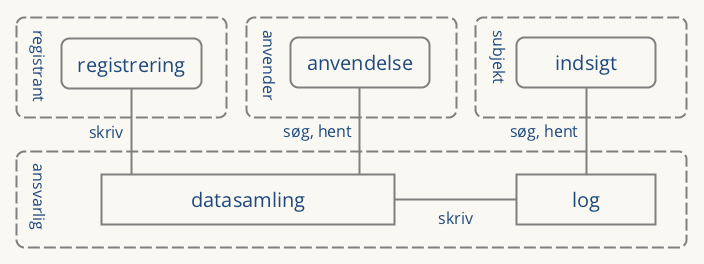
\includegraphics{figures/use-direct.png}
\caption{Implementeringsmønster med direkte adgang til registre}
\end{figure}

I dette mønster, som er simpelt og måske det mest klassiske, er det
\texttt{dataansvarlig}, der selv udstiller data til de mulige anvendere
via en service-orienteret arkitektur. \texttt{Dataansvarlig} er også
ansvarlig for at betjene \texttt{datasubjektets} forespørgsler om
\texttt{datansvarligs} brug af personlige data.

Fordelen ved dette mønster er, at det er simpelt. Ulempen er, at
\texttt{dataansvarlig} kommer til at bære hele udgiften ved at stille
data bredt til rådighed.

\paragraph{Datadistribution}\label{datadistribution}

\begin{figure}
\centering
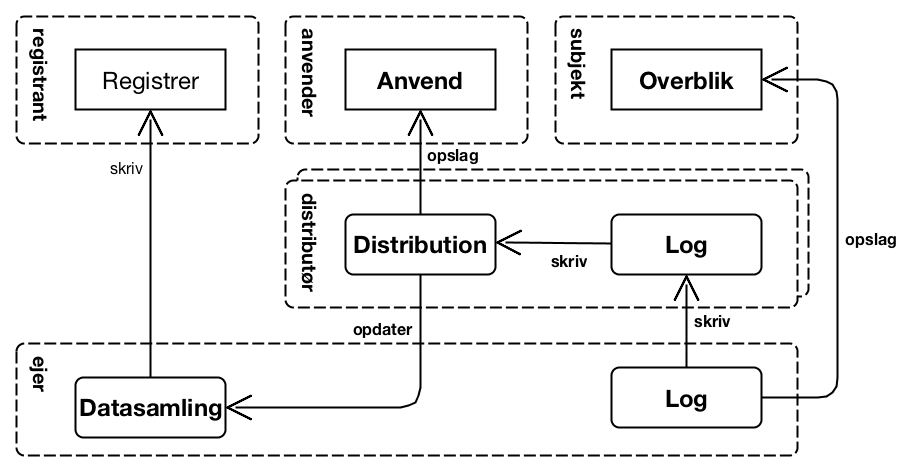
\includegraphics{figures/use-dist.png}
\caption{Implementeringsmønster for datadistribution}
\end{figure}

I dette mønster er \texttt{dataansvarlig} fortsat ansvarlig for at
tilbyde en service til registrering af data. Anvendelsesdelen er
imidlertid afløftet til en \texttt{datadistributør} (evt. flere). Dette
giver \texttt{datadistributøren} mulighed for at fokusere netop på
distributionen, dvs. at gøre data bredt tilgængeligt (dog naturligvis
under håndhævelse af adgangskrav specificeret af \texttt{dataejer}) til
\texttt{dataanvendere}.

Når nye data registreres, har \texttt{dataansvarlig} ansvaret for at
opdatere \texttt{kopien} af \texttt{datasamlingen} hos
\texttt{datadistributøren}.

I det tilfælde, hvor ensartede \texttt{datasamlinger} ligger hos flere,
separate \texttt{dataansvarlige} - eksempelvis sundhedsdata opbevaret i
forskellige regioner - er det fordelagtigt at anvende et \texttt{index}
for at sikre effektive opslag. \texttt{Dataansvarlig} opdaterer dette
\texttt{index}, når en \texttt{registrant} opdaterer
\texttt{datasamlingen}.

Logningsmæssigt er den enkelte \texttt{distributør} ansvarlig for at
logge \texttt{dataanvenders} adgang til data. Samtidig er den enkelte
\texttt{distributør} ansvarlig for at sørge for konsolidering af loggen
for at sikre, at \texttt{datasubjekt} har adgang til information om
anvendelse af data om vedkommende selv. I figuren er log-konsolidering
lagt hos \texttt{dataansvarlig}, men den kunne i princippet også være
uddelegeret - så længe, der er et entydigt og klart \emph{single point
of contact} for \texttt{datasubjektets} opslag i anvendelsen af
personlige data.

\paragraph{Distribueret service- og
data-platform}\label{distribueret-service--og-data-platform}

\begin{figure}
\centering
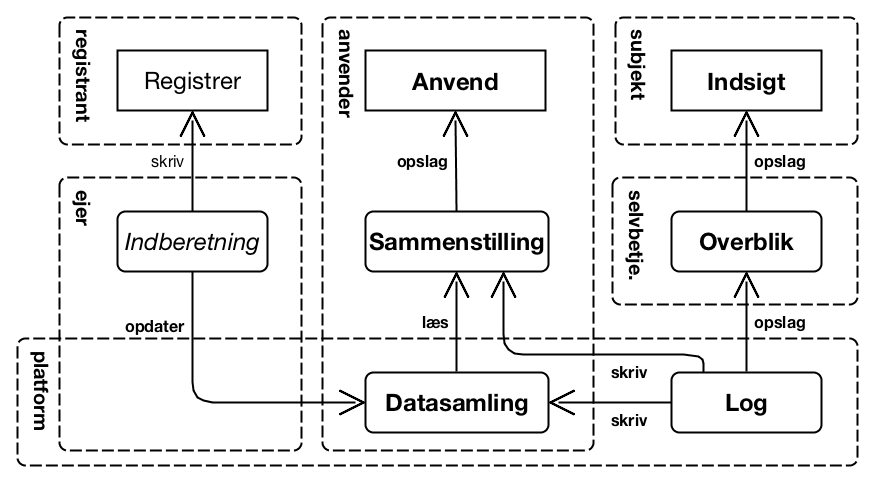
\includegraphics{figures/use-plat.png}
\caption{Implementeringsmønster for distribueret dataplatform}
\end{figure}

Delingsansvaret er i dette mønster i høj grad håndteret af en
\texttt{dataplatform}. Platformen er distribueret og er i stand til at
replikere data på tværs af \texttt{dataansvarlige}og
\texttt{dataanvendere}. Dvs., at data, der registreres via en
\texttt{dataansvarlig} myndighed, gøres tilgængelige for andre,
dataanvendende myndigheder via platformen.

Da \texttt{dataplatformen} kan rumme data fra mange forskellige
\texttt{dataejere}, muliggøres effektiv sammenstiling af data hos
\texttt{dataanvenderen}, der kan kombinere \texttt{data} fra
\texttt{egne\ samlinger} med \texttt{data} fra andre \texttt{samlinger}.
\texttt{Data} kan her forstås både som simple opslag i egne eller andres
\texttt{datasamlinger}, og som sammenstillinger, hvor data fra flere
\texttt{samlinger} kombineres for at servicere \texttt{dataanvenders}
applikationer.

Platformen er ansvarlig for at håndhæve adgangskontrol, herunder at
sikre, at anvendelsesapplikationer har den nødvendige lovhjmmel til at
tilgå en given, distribueret \texttt{samling}. Eventuelle services hos
\texttt{dataanvender}, der gør brug af data, er ansvarlige for at logge
deres brug. Platformen konsoliderer brugs-loggen og gør det muligt for
\texttt{datasubjekt} at få overblik over brug af personlige data.

Fordelen ved dette mønster er den umiddelbare og standardiserede
tilgænglighed til data, som en \texttt{dataplatform} kan levere. Ulempen
er, at kompleksiteten øges, samt at der stilles større krav til
\texttt{dataanvenders} modenhed ift. den tekniske adgang til data (da
\texttt{dataanvenders} applikationer i praksis vil skulle afvikles på
den distribuerede Service- og Dataplatform).

\emph{(Uafklaret: Skal Dataanvenders applikationer/services have direkte
adgang til distribuerede data, eller skal adgang fortsat ske via et
servicesnit, der kan varetage adgangskontol m.m.? Tracket i issue 7.)}

\subsubsection{Registreret forsendelse}\label{registreret-forsendelse}

Når en myndighed vil initiere en specifik og målrettet datadeling - dvs.
sende data (herunder dokumenter) til en anden myndighed, virksomhed
eller borger - kan det ske via ét af de tre nedenstående mønstre.

\paragraph{Sikker e-mail}\label{sikker-e-mail}

\begin{figure}
\centering
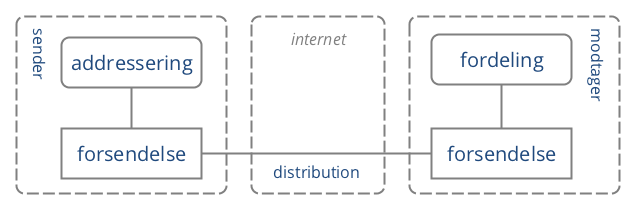
\includegraphics{figures/send-email.png}
\caption{Implementeringsmønster for Sikker e-mail}
\end{figure}

Et meget anvendt mønster for myndighed til myndighed-kommunikation er at
levere en \texttt{meddelelse} fra \texttt{afsender} til
\texttt{modtager} gennem \texttt{forsendelse} brug af sikker e-mail. Ud
over at påpege, at \texttt{distributionen} her sker via en sikker og
krypteret forbindelse, faldet detr uden for dette dokuments scope at
beskrive dette mønster yderligere. Det er dog medtaget for reference
pga. dets brede anvendelse. Det er endvidere oplagt at betragte dette
mønster som et særtilfælde af det generelle `Service provider'-mønster
nedenfor.

Fordelen ved dette mønster er, at det er simpelt og benytter sig af
standardteknologi. Ulempen er, at det kun dækker myndighed til
myndighed-kommunikation. Derudover sætter standardteknologien (e-mail)
visse begrænsninger for funktionalitet, der fx understøtter
\texttt{fordeling}(automatisk routing) af beskeder hos modtagende
virksomhed/myndighed i det tilfælde, hvor \texttt{meddelelsen} ikke har
én specifik \texttt{modtager}.

\paragraph{Fælles system}\label{fuxe6lles-system}

\begin{figure}
\centering
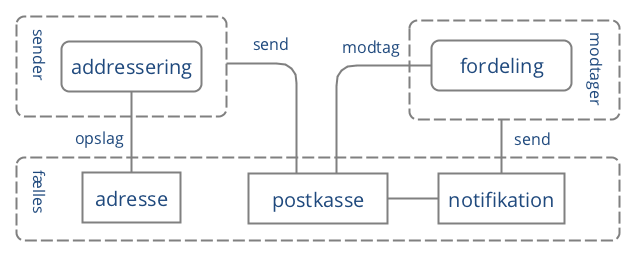
\includegraphics{figures/send-shared.png}
\caption{Implementeringsmønster for fælles system}
\end{figure}

Ved brug af Fælles system-mønsteret til forsendelse af en
\texttt{meddelelse} benytter \texttt{afsender} og \texttt{modtager} et
centralt, fælles \texttt{postkasse} til hhv. at placere
\texttt{meddelelsen} og læse den. I den analoge verden svarer dette
mønster til, at \texttt{afsender} og \texttt{modtager} benytter et
fælles postbokskontor. Digitalt er dette mønster fx implementeret af
Digital Post, hvor såvel myndigheder, virksomheder og borgere kan
placere \texttt{meddelelser}, der efterfølgende kan hentes af
\texttt{modtager}. Også messaging-funktionaliteten i mange af de sociale
medieplatforme (fx Facebook) falder i denne kategori.

TIl forskel fra Sikker e-mail-mønsteret ovenfor er Fælles
system-mønsteret mere robust, både da \texttt{adresseringsservicen}
tilbyder opslag/verifikation mod et \texttt{adresseregister}, samt da
\texttt{meddelelsen} opbevares i infrastrukturen, indtil
\texttt{modtager} aktivt læser den - i modsætning til Sikker e-mail,
hvori infrastrukturen blot videresender \texttt{meddelelsen} og dermed
er afhængig af, at \texttt{modtageren} i praksis findes.

\texttt{Postkassefunktionaliteten} har endvidere mulighed for at trække
på en \texttt{notifikationsservice}, der kan tilbyde indholdsreducerede
notifikationer til \texttt{modtager} om den nye \texttt{meddelelse}.

Et Fælles system-mønster kan fungere på mange niveauer, herunder
nationalt (fx Digital Post); inden for et specifikt domæne, fx på
sundhedsområdet; eller rent bilateralt, hvor to organisationer enes om
dette mønster og vælger en passende meddelelsesplatform.

\paragraph{Økosystem/Service
providers}\label{uxf8kosystemservice-providers}

\begin{figure}
\centering
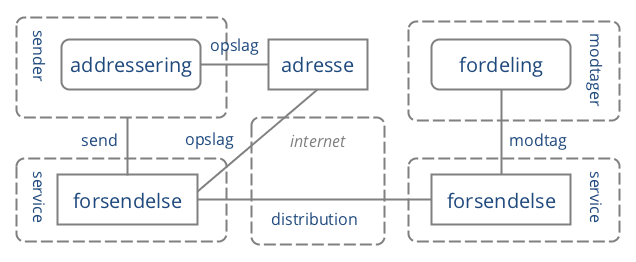
\includegraphics{figures/send-eco.png}
\caption{Implementeringsmønster for økosystem}
\end{figure}

I dette mønster deltager både \texttt{afsender} (A) og \texttt{modtager}
(D) i et \texttt{meddelelses}-økosystem ved at vælge hver sin
Forsendelses-Service provider (hhv. B og C). Økosystem-mønsteret er
bl.a. kendt i kontekst af den europæiske eDelivery-standard som en
\emph{four corner model}.

Et fælles \texttt{adresseregister/kontaktregister} udgør en central
komponent i økosystemet, der gør det muligt for alle parter at slå den
relevante adresseringsinformation op. En \texttt{afsender} kan via
\texttt{adresseregisteret} se/verificere mulige \texttt{modtagere}, samt
evt. afgøre hvilken konkrete meddelelsesformater/kanaler,
\texttt{modtager} kan håndtere. \texttt{Forsendelsesservicen}, der
håndterer afsendelse af Meddelelsen, kan benytte
\texttt{adresseregisteret} til at finde \texttt{modtagerens} konkrete
\texttt{Service\ provider} og bliver dermed i stand til at levere
\texttt{meddelelsen}.

Mønsteret vil typisk være symmetrisk, således at en \texttt{afsender}
også kan indgå som \texttt{modtager} og vice versa. Mønsteret kan i
øvrigt både være generisk eller specifikt for et domæne, der fx kan
stille ekstra krav til \texttt{meddelelsens} format.

Fordelene ved Økosystem-mønsteret er, at det er robust, fleksibelt og
løbende kan udvides med nye \texttt{Service\ providers}. Ulempen er, at
der stilles store krav til det centrale \texttt{adresseregister}, samt
at der fortsat ikke findes standardteknologier, der dækker mønsteret.

\subsubsection{Registrering}\label{registrering}

Registrering af data er ikke i scope for denne referencearkitektur, men
medtages kort pga. sin væsentlige relation til Indeks-konceptet.

\emph{Opdateres.}

\begin{description}
\tightlist
\item[Ansvar hos registrant]
\emph{implementationsmønster}
\item[Ansvar hos dataejer]
\emph{implementationsmønster}
\item[Ansvar hos distributør]
\emph{implementationsmønster}
\end{description}

\subsection{Integrationer}\label{integrationer}

I de ovenstående implementeringsmønstre for hhv. Anvendelse af
udstillede data og Registreret forsendelse indgår der en lang række
relationer mellem de beskrevne elementer. Relationerne dækker i praksis
over integrationer mellem to applikationer. Nedenfor opridser vi de
relationer, der er væsentlige for denne referencearkitektur. Alle
relationer er ikke relevante i vores kontekst - men sagt populært, hvis
der ``står noget på en linje mellem to kasser'', er de mest fremtrædende
karakteristika og kendetegn ved den underliggende integration beskrevet
nedenfor:

\emph{Integrationsbeskrivelser opdateres.}

\begin{description}
\tightlist
\item[skriv]
Med kvittering\ldots{}
\item[opslag]
beskytter mod misbrug, og beskyttet mod DDOS
\end{description}

\emph{TBU: DNS}

\begin{description}
\tightlist
\item[opdater]
Bulk, Delta, Teknologispecifikt
\item[konsolider]
Skriv eller høst
\item[læs]
SQL eller Fil, men log
\item[distribution]
uafviselighed, beskyttet, payload/header
\item[hent meddelelse]
\emph{TBU}
\item[modtag notifikation]
borger - SMS/APP
\end{description}

\subsection{Områder for
standardisering/profileringer}\label{omruxe5der-for-standardiseringprofileringer}

Nedenstående, tekniske områder er kandidater til at indgå i
referencearkitekturen i forhold til at pege på en anbefalet standard
eller en særlig profilering, evt. vendt mod de enkelte, tekniske
mønstre.

Integrationer - Service Design Guidelines

\begin{itemize}
\tightlist
\item
  Data Write Protocols
\item
  Data Access Protocols
\item
  Distribution Protocols
\item
  Notification Protocols
\item
  Synchronisation Protocols
\end{itemize}

Indholdsmæssige standarder - Metadata for opslag/søgning/anvendelse -
Log format - Hjemmel (samtykke, lov) - Kontekts (klassifkation af
anvendelse) - Hændelsesbeskeder - Identifikation - Klassifikation af
følsomhed

\subsection{Identifikation af eksisterende
standarder}\label{identifikation-af-eksisterende-standarder}

\emph{TBU.}
